\chapter{肌肉与关节}\label{ch:g10:muscles-and-joints}

一名足球运动员踩稳脚、转身，随即抱着膝盖倒地。
一小时后，诊断结果出来：\omterm{def:g10:muscles-and-joints:joint}{韧带}撕裂。骨头
没有折断，肌肉也没有受损；一条长仅几厘米的组织带，
其功能是使两块骨头保持对齐，却在一次它从未能承受的扭转下断裂。
要弄清撕裂的原因，以及膝\omterm{def:g10:muscles-and-joints:joint}{关节}为何需要
数月才能恢复，就得了解\omterm{def:g10:muscles-and-joints:joint}{关节}的构造、肌肉如何牵拉\omterm{def:g10:muscles-and-joints:joint}{关节}，
以及一个重七十
千克的人单腿落地时，\omterm{def:g10:muscles-and-joints:joint}{关节}内部会受到怎样的力。

\section{关节}

\begin{definition}[关节]\label{def:g10:muscles-and-joints:joint}
\emph{关节}\index{关节}是两块骨头相接的部位。在
膝、髋、肩或肘等可活动关节中，骨端覆盖着一层光滑的
\emph{软骨}\index{软骨}，厚几毫米，
并包在一个密闭的囊中，即
\emph{关节囊}，其内衬分泌
润滑关节表面的\emph{滑液}。坚韧的组织带，即
\emph{韧带}\index{韧带}，横跨关节，从一块骨延伸至另一块，
将关节运动限制在正常范围之内。在膝关节中，
两片弯月形的软骨，即\emph{半月板}，位于两骨之间，
起分散负荷的作用。
\end{definition}

\begin{omfigure}
\begin{tikzpicture}
  \node[anchor=south west, inner sep=0] (img) at (0,0)
    {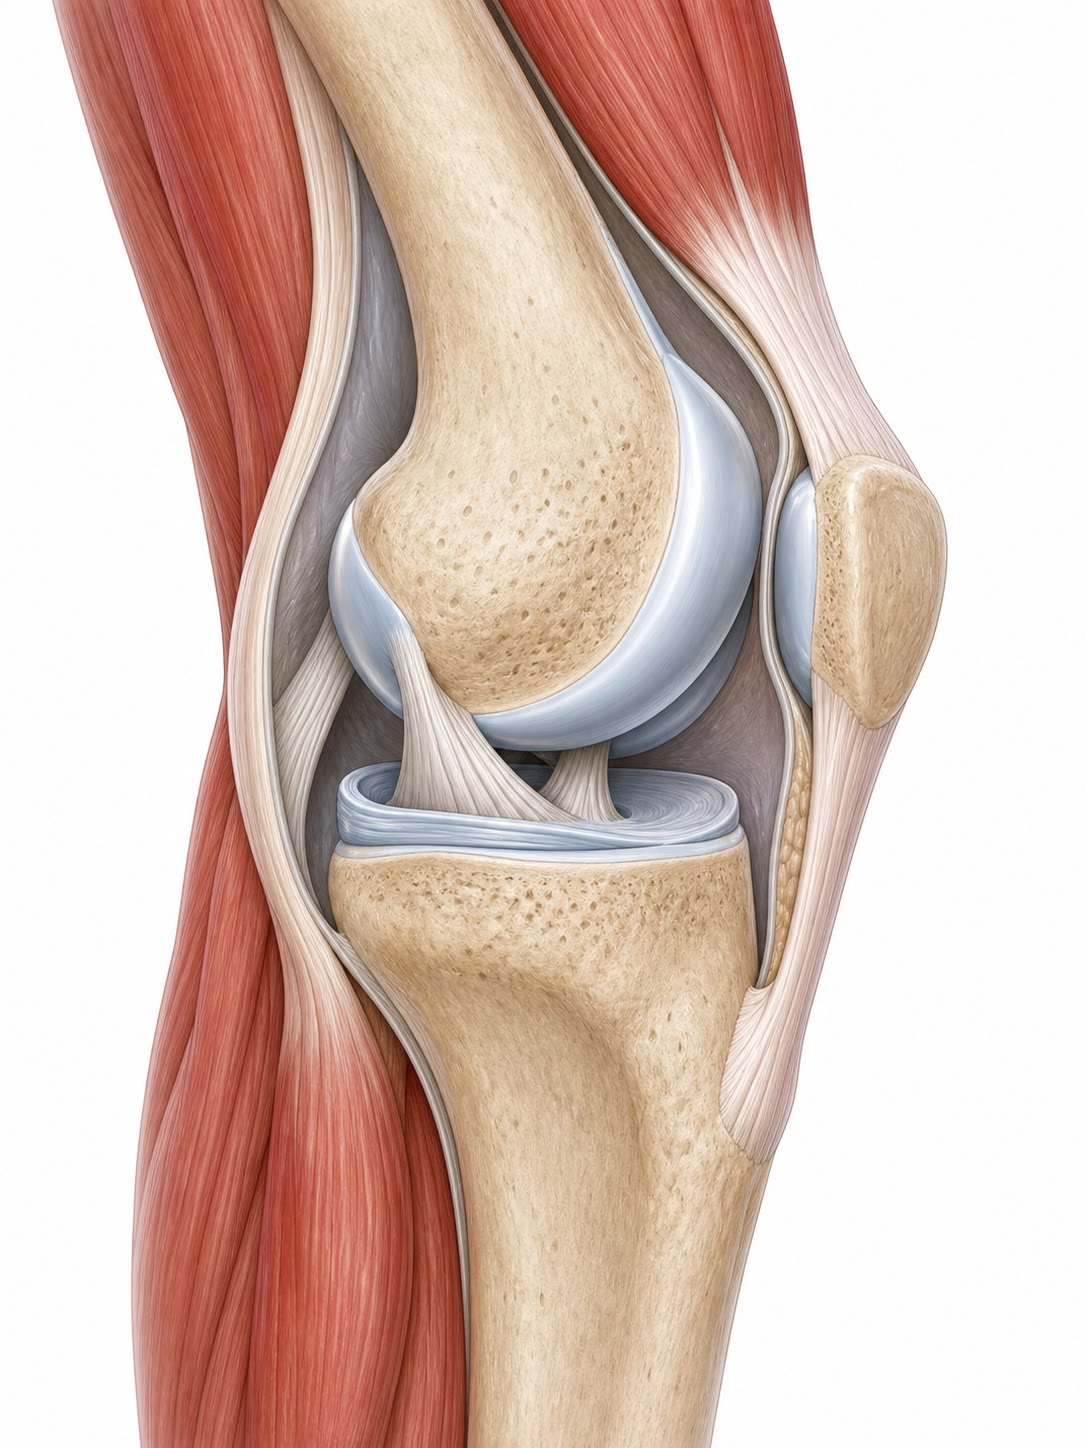
\includegraphics[width=0.4\linewidth]{images/book2/ai/fig-knee-cutaway.jpg}};
  \begin{scope}[x={(img.south east)}, y={(img.north west)},
      every node/.style={font=\small}]
    \draw[omDef, thick] (0.50,0.86) -- (1.05,0.90) node[right] {股骨};
    \draw[omDef, thick] (0.76,0.74) -- (1.05,0.74) node[right] {股四头肌腱};
    \draw[omDef, thick] (0.82,0.58) -- (1.05,0.58) node[right] {髌骨};
    \draw[omDef, thick] (0.50,0.20) -- (1.05,0.14) node[right] {胫骨};
    \draw[omDef, thick] (0.34,0.60) -- (-0.05,0.64) node[left] {软骨};
    \draw[omDef, thick] (0.50,0.50) -- (-0.05,0.50) node[left] {韧带};
    \draw[omDef, thick] (0.40,0.44) -- (-0.05,0.36) node[left] {半月板};
  \end{scope}
\end{tikzpicture}

{\small 膝\omterm{def:g10:muscles-and-joints:joint}{关节}剖面：股骨在上，胫骨在下，髌骨
（膝盖骨）位于前方，嵌在大腿肌肉的\omterm{def:g10:muscles-and-joints:muscle}{肌腱}中；骨端覆盖\omterm{def:g10:muscles-and-joints:joint}{软骨}，
两骨之间为半月板，\omterm{def:g10:muscles-and-joints:joint}{韧带}将骨
连在一起。}
\end{omfigure}

\begin{proposition}[各部分的作用]\label{prop:g10:muscles-and-joints:parts}
\omterm{def:g10:muscles-and-joints:joint}{软骨}和滑液使\omterm{def:g10:muscles-and-joints:joint}{关节}面之间的滑动
摩擦远小于冰面与冰面之间的摩擦；半月板分散本会
集中于几平方毫米上的负荷；\omterm{def:g10:muscles-and-joints:joint}{韧带}允许
膝\omterm{def:g10:muscles-and-joints:joint}{关节}屈伸，却能抵抗扭转和侧向
弯曲；\omterm{def:g10:muscles-and-joints:joint}{关节}囊将滑液封存在内。每个部分各有其损伤方式：
\omterm{def:g10:muscles-and-joints:joint}{软骨}会磨损（\omterm{def:g10:muscles-and-joints:joint}{关节}病），半月板在膝\omterm{def:g10:muscles-and-joints:joint}{关节}弯曲时受扭转而撕裂，
\omterm{def:g10:muscles-and-joints:joint}{韧带}则在\omterm{def:g10:muscles-and-joints:joint}{关节}被
迫超出活动范围时扭伤或断裂。
\end{proposition}
\admitted

\begin{example}[扭伤、撕裂、脱位]\label{ex:g10:muscles-and-joints:injuries}
在路缘石上扭伤脚踝：外侧\omterm{def:g10:muscles-and-joints:joint}{韧带}被拉伸
超过其极限——即\emph{扭伤}；\omterm{def:g10:muscles-and-joints:joint}{关节}囊出血，\omterm{def:g10:muscles-and-joints:joint}{关节}随之肿胀，积液增多。
在身体未热身时猛拉股后肌群，部分
\omterm{def:g10:muscles-and-joints:muscle}{肌纤维}断裂，即肌肉\emph{撕裂}。伸手撑地摔倒时，
肱骨头可能脱出\omterm{def:g10:muscles-and-joints:joint}{关节}窝，即
\emph{脱位}，\omterm{def:g10:muscles-and-joints:joint}{韧带}与\omterm{def:g10:muscles-and-joints:joint}{关节}囊在此过程中被拉伸或撕裂。
这些损伤都不是骨折，但恢复时间可能比骨折更长。
\end{example}

\section{肌肉成对牵拉}

\begin{definition}[骨骼肌与肌腱]\label{def:g10:muscles-and-joints:muscle}
\emph{骨骼肌}\index{骨骼肌}是由
数千条细长的\omterm{def:g10:cells-common-unit:cell}{细胞}，即\emph{肌纤维}，聚集成束而构成的器官；
每条肌纤维受神经刺激时缩短。肌肉的两端
逐渐变细，形成\emph{肌腱}\index{肌腱}，即一条
不能收缩、附着于骨的组织索。肌肉只能
以缩短的方式\emph{牵拉}，且只能沿其自身长度方向作用：它通过牵拉
\omterm{def:g10:muscles-and-joints:joint}{关节}另一侧的骨来带动\omterm{def:g10:muscles-and-joints:joint}{关节}运动。
\end{definition}

\begin{proposition}[拮抗肌对]\label{prop:g10:muscles-and-joints:antagonists}
肌肉只能拉而不能推，因此\omterm{def:g10:muscles-and-joints:joint}{关节}的每一次运动都需要两块或两组
作用相反的肌肉或肌群：一块\emph{屈肌}使\omterm{def:g10:muscles-and-joints:joint}{关节}弯曲，
一块\emph{伸肌}使其伸直。当其中一块
收缩时，另一块舒张并被拉长；要保持某一姿势，
两者须同时收缩。肱二头肌屈肘，肱三头肌伸肘；
大腿前侧的股四头肌伸膝，
后侧的股后肌群屈膝。
\end{proposition}
\admitted

\begin{omfigure}
\begin{tikzpicture}[>=Stealth, font=\small, line cap=round]
  % upper arm (humerus) horizontal, forearm angled
  \draw[line width=7pt, gray!45] (0,0) -- (5,0);         % humerus
  \draw[line width=6pt, gray!45] (5,0) -- (8.6,2.0);     % forearm
  \fill[gray!60] (5,0) circle (0.28);
  \node[anchor=north] at (2.5,-0.25) {肱骨};
  \node[anchor=north west] at (7.2,1.1) {前臂};
  \node[anchor=west] at (5.5,-0.5) {肘};
  % biceps: from shoulder region above humerus to forearm just past elbow
  \draw[line width=9pt, omThm!60] (0.6,0.6) .. controls (3,1.4) .. (5.35,0.9);
  \draw[thick, omThm!80!black] (5.35,0.9) -- (5.65,0.45);   % tendon
  \node[omThm!80!black, anchor=south] at (3,1.3) {肱二头肌（屈肌）：收缩};
  % triceps: below humerus to the back of the forearm
  \draw[line width=7pt, omDef!50] (0.6,-0.9) .. controls (3,-1.6) .. (4.9,-1.0);
  \draw[thick, omDef!80!black] (4.9,-1.0) -- (5.25,-0.4);
  \node[omDef!80!black, anchor=north] at (3,-1.65) {肱三头肌（伸肌）：舒张，被拉长};
  \draw[->, thick] (8.6,2.0) to[bend right=20] (8.0,3.0);
  \node[anchor=south] at (8.3,3.05) {屈曲};
  \draw[->, thick, omThm!80!black] (5.65,0.45) -- (5.2,0.75);
\end{tikzpicture}

{\small 肘部的一对拮抗肌。肱二头肌附着于紧靠\omterm{def:g10:muscles-and-joints:joint}{关节}的前臂上，
收缩使肘部弯曲；肱三头肌附着于\omterm{def:g10:muscles-and-joints:joint}{关节}后方，舒张并被拉长。
互换二者的角色，
即可伸直手臂。}
\end{omfigure}

\begin{proposition}[杠杆与力]\label{prop:g10:muscles-and-joints:lever}
在\omterm{def:g10:muscles-and-joints:joint}{关节}处转动的骨即为一根杠杆。\omterm{def:g10:muscles-and-joints:muscle}{肌腱}附着于距支点较近处，距离为 $d$，
负载作用于距支点较远处，距离为 $D$；要保持平衡，
肌肉的拉力须为
\[
F_{\text{肌肉}} = F_{\text{负载}} \times \frac{D}{d},
\]
所需的力是负载的数倍。这种结构以力换速度和
活动范围：肌肉的微小缩短即可使
手或脚产生大幅、快速的运动，
代价是\omterm{def:g10:muscles-and-joints:muscle}{肌腱}和\omterm{def:g10:muscles-and-joints:joint}{关节}承受很大的力。
\end{proposition}
\admitted

\begin{example}[提着一只袋子]\label{ex:g10:muscles-and-joints:bag}
一只 \qty{5}{kg} 的袋子（重 \qty{49}{N}）挂在手上，
距肘 \qty{35}{cm}；肱二头肌\omterm{def:g10:muscles-and-joints:muscle}{肌腱}的附着点距肘 \qty{5}{cm}，
肱二头肌的拉力为 $49 \times 35/5 = \qty{343}{N}$ ——
是负载的七倍，相当于 \qty{35}{kg} 的重量——而肘\omterm{def:g10:muscles-and-joints:joint}{关节}
受到的挤压力约为 \qty{300}{N}。肌肉、\omterm{def:g10:muscles-and-joints:muscle}{肌腱}和\omterm{def:g10:muscles-and-joints:joint}{软骨}
本就为承受这些力而构造；真正损伤它们的，
是方向错误的突然受力，
或是超出组织修复能力的反复负载。
\end{example}

\begin{omfigure}
\begin{tikzpicture}[>=Stealth, font=\small]
  \draw[line width=6pt, gray!45] (0,0) -- (7,0);
  \fill[gray!70] (0,0) circle (0.25);
  \node[anchor=north] at (0,-0.35) {肘（支点）};
  \draw[->, very thick, omThm] (1,0.15) -- (1,2.2) node[above] {$F_{\text{肌肉}}$};
  \draw[->, very thick, omDef] (7,-0.15) -- (7,-1.6) node[below] {$F_{\text{负载}} = \qty{49}{N}$};
  \draw[<->] (0,0.9) -- (1,0.9) node[midway, above, xshift=-4mm] {$d = \qty{5}{cm}$};
  \draw[<->] (0,-1.25) -- (7,-1.25) node[midway, below] {$D = \qty{35}{cm}$};
\end{tikzpicture}

{\small 前臂作为杠杆：肱二头肌在靠近支点处牵拉，
负载悬挂于远离支点处。$F_{\text{肌肉}} \times d =
F_{\text{负载}} \times D$，因此肌肉的力为
负载的 $D/d = 7$ 倍。}
\end{omfigure}

\section{肌肉内部}

\begin{proposition}[肌纤维的结构]\label{prop:g10:muscles-and-joints:fibre}
\omterm{def:g10:muscles-and-joints:muscle}{肌纤维}是一个巨大的单\omterm{def:g10:cells-common-unit:cell}{细胞}，宽 \num{10}--\qty{100}{\micro m}，
长可达数厘米，内含许多\omterm{def:g10:cells-common-unit:organelle}{细胞核}。其内部
充满平行排列的\emph{肌原纤维}，每条肌原纤维是一串重复单元，
其中粗、细两种\omterm{def:g10:chemistry-of-life:families}{蛋白质}丝相互交错。
收缩即细丝在粗丝之间滑动，
由 ATP 驱动：每个单元缩短一部分，
肌原纤维的缩短为各单元之和，\omterm{def:g10:muscles-and-joints:muscle}{肌纤维}随之缩短。位于
肌原纤维之间的\omterm{def:g10:cells-common-unit:organelle}{线粒体}提供 ATP；每条\omterm{def:g10:muscles-and-joints:muscle}{肌纤维}上的神经末梢
发出收缩的指令。
\end{proposition}
\admitted

\begin{omfigure}
\begin{tikzpicture}[font=\small, >=Stealth]
  \tikzset{lvl/.style={draw, rounded corners, thick, align=center, minimum height=1.1cm}}
  \node[lvl, fill=omThm!12, text width=2.1cm] (m) at (0,0) {肌肉 \\（器官）};
  \node[lvl, fill=omThm!12, text width=2.1cm] (b) at (3.0,0) {肌束};
  \node[lvl, fill=omProp!15, text width=2.1cm] (f) at (6.0,0) {肌纤维 \\（一个细胞）};
  \node[lvl, fill=omDef!12, text width=2.1cm] (my) at (9.0,0) {肌原纤维};
  \node[lvl, fill=omMeth!15, text width=2.1cm] (fi) at (12.0,0) {粗丝和细丝};
  \foreach \a/\b in {m/b, b/f, f/my, my/fi} \draw[->] (\a) -- (\b);
  \node[anchor=north, font=\scriptsize] at (m.south) {厘米};
  \node[anchor=north, font=\scriptsize] at (b.south) {毫米};
  \node[anchor=north, font=\scriptsize] at (f.south) {宽 \qty{50}{\micro m}};
  \node[anchor=north, font=\scriptsize] at (my.south) {宽 \qty{1}{\micro m}};
  \node[anchor=north, font=\scriptsize] at (fi.south) {\qty{10}{nm}};
\end{tikzpicture}

{\small 从整块肌肉到使其缩短的分子，共有五个层级，
每一层都由下一层聚集而成。细丝彼此滑动，
并在每个单元中重复发生，
即为收缩。}
\end{omfigure}

\begin{definition}[纤维类型]\label{def:g10:muscles-and-joints:types}
\omterm{def:g10:muscles-and-joints:muscle}{肌纤维}主要分为两类。\emph{慢\omterm{def:g10:muscles-and-joints:muscle}{肌纤维}}收缩缓慢而力弱，
但持久不疲：\omterm{def:g10:cells-common-unit:organelle}{线粒体}和毛细血管丰富，
含储氧\omterm{def:g10:chemistry-of-life:families}{蛋白质}而呈红色，主要依靠呼吸作用供能，
常见于姿势肌和耐力运动员的肌肉中。\emph{快\omterm{def:g10:muscles-and-joints:muscle}{肌纤维}}收缩迅速、
力量强大，但不到一分钟即疲劳：\omterm{def:g10:cells-common-unit:organelle}{线粒体}较少，颜色较浅，
主要依赖磷酸盐储备和\omterm{def:g10:cell-metabolism:fermentation}{发酵}供能，常见于短跑运动员。
某块肌肉中两类纤维的比例很大程度上是遗传的；
训练更多改变纤维的大小和“配备”，
而非其数量。
\end{definition}

\begin{example}[读取肌肉活检结果]\label{ex:g10:muscles-and-joints:biopsy}
对大腿肌肉薄片进行\omterm{def:g10:cells-common-unit:organelle}{线粒体}酶染色，
结果呈镶嵌状：深色纤维（慢肌）与浅色纤维（快肌）相间。马拉松
跑者的样本中深色纤维占 80\%；短跑运动员为 30\%；未经训练者
约各占一半。同一位跑者经过一年短跑训练后，
同样染色显示浅色纤维增大，但数量并未增多。
\end{example}

\section{疲劳、损伤与修复}

\begin{proposition}[肌肉的极限]\label{prop:g10:muscles-and-joints:limits}
肌肉以三种不同方式失效。\emph{疲劳}：当 ATP 供应
跟不上时，力量下降——快\omterm{def:g10:muscles-and-joints:muscle}{肌纤维}在一分钟内，
慢\omterm{def:g10:muscles-and-joints:muscle}{肌纤维}则需数小时——
休息后可恢复。\emph{痉挛}：突发、持续且不由自主的收缩，
常由脱水或失盐引起。\emph{损伤}：纤维受力超过其强度而撕裂，
多发生于肌肉寒冷、疲劳或收缩时被拉长的情况下。
纤维可在数周内由肌肉中的储备\omterm{def:g10:cells-common-unit:cell}{细胞}修复；
\omterm{def:g10:muscles-and-joints:muscle}{肌腱}或\omterm{def:g10:muscles-and-joints:joint}{韧带}血液供应较差，
需数月才能修复。
\end{proposition}
\admitted

\begin{method}[分析肌肉骨骼损伤]\label{met:g10:muscles-and-joints:analyse}
\begin{enumerate}
  \item 判断造成损伤的运动及其方向：\omterm{def:g10:muscles-and-joints:joint}{关节}
        是在活动范围之内运动（肌肉问题），
        还是超出范围（\omterm{def:g10:muscles-and-joints:joint}{韧带}或\omterm{def:g10:muscles-and-joints:joint}{关节}囊问题）？
  \item 判断受损组织：\omterm{def:g10:muscles-and-joints:muscle}{肌纤维}撕裂（肌腹疼痛、
        无力）；\omterm{def:g10:muscles-and-joints:joint}{韧带}扭伤（\omterm{def:g10:muscles-and-joints:joint}{关节}处疼痛、肿胀，
        \omterm{def:g10:muscles-and-joints:joint}{关节}不稳）；\omterm{def:g10:muscles-and-joints:muscle}{肌腱}在反复负荷下发炎；
        \omterm{def:g10:muscles-and-joints:joint}{软骨}则多年间悄然磨损。
  \item 估算作用力：运用杠杆规则；
        需注意着地或制动时，作用力可达体重的数倍。
  \item 根据组织的血液供应预测恢复时间：
        肌肉需数周，\omterm{def:g10:muscles-and-joints:joint}{韧带}与\omterm{def:g10:muscles-and-joints:muscle}{肌腱}需数月，
        \omterm{def:g10:muscles-and-joints:joint}{软骨}几乎不能恢复。
\end{enumerate}
\end{method}

\begin{remark}[为何热身有效]\label{rem:g10:muscles-and-joints:warmup}
十分钟的轻柔活动可使肌肉温度升高一到两度，
从而使肌肉\omterm{def:g10:chemistry-of-life:families}{蛋白质}更易伸展、酶的反应更快；
它还使毛细血管开放，以输送
\cref{ch:g10:heart-lungs-effort}中所述的氧气，并使\omterm{def:g10:muscles-and-joints:joint}{软骨}表面的滑液膜增厚。
冷的肌肉若被要求做最大收缩，
是撕裂最常见的原因；
\omterm{def:g10:muscles-and-joints:joint}{关节}在滑液尚未铺开时便承受负荷，磨损更快。
\end{remark}

\section{练习}

\begin{exercise}[$\star$]\label{exo:g10:muscles-and-joints:1}
说出可动\omterm{def:g10:muscles-and-joints:joint}{关节}的各组成部分，并说明各部分的作用。
\end{exercise}

\begin{exercise}[$\star$]\label{exo:g10:muscles-and-joints:2}
\omterm{def:g10:muscles-and-joints:muscle}{肌腱}与\omterm{def:g10:muscles-and-joints:joint}{韧带}有何区别？
\end{exercise}

\begin{exercise}[$\star$]\label{exo:g10:muscles-and-joints:3}
为何每个\omterm{def:g10:muscles-and-joints:joint}{关节}至少需要两块肌肉才能运动？
\end{exercise}

\begin{exercise}[$\star$]\label{exo:g10:muscles-and-joints:4}
区分扭伤、肌肉撕裂与脱位，
依据是各自所涉及的组织。
\end{exercise}

\begin{exercise}[$\star$]\label{exo:g10:muscles-and-joints:5}
比较慢\omterm{def:g10:muscles-and-joints:muscle}{肌纤维}与快\omterm{def:g10:muscles-and-joints:muscle}{肌纤维}，给出两点差异。
\end{exercise}

\begin{exercise}[$\star\star$]\label{exo:g10:muscles-and-joints:6}
手中握着一个 \qty{2}{kg} 的哑铃，
哑铃距肘 \qty{32}{cm}，二头肌附着点距哑铃 \qty{4}{cm}。
求二头肌中的作用力（$g = \qty{9.8}{N/kg}$）。
\end{exercise}

\begin{exercise}[$\star\star$]\label{exo:g10:muscles-and-joints:7}
说明为何二头肌与三头肌都必须收缩，
才能使手臂在不可预料的推力下保持静止。
\end{exercise}

\begin{exercise}[$\star\star$]\label{exo:g10:muscles-and-joints:8}
一根长 \qty{3}{cm} 的\omterm{def:g10:muscles-and-joints:muscle}{肌纤维}收缩时
缩短 20\%。若该纤维的\omterm{def:g10:muscles-and-joints:muscle}{肌腱}附着点距肘
\qty{5}{cm}，手距肘 \qty{35}{cm}，则手移动了多少？
\end{exercise}

\begin{exercise}[$\star\star$]\label{exo:g10:muscles-and-joints:9}
为何肩\omterm{def:g10:muscles-and-joints:joint}{关节}这一全身活动度最大的\omterm{def:g10:muscles-and-joints:joint}{关节}，
也是最常脱位的\omterm{def:g10:muscles-and-joints:joint}{关节}？
\end{exercise}

\begin{exercise}[$\star\star$]\label{exo:g10:muscles-and-joints:10}
一名跑步者在炎热赛事的终点处小腿肌肉痉挛。
请依据本章提出两个原因及一种处理方法。
\end{exercise}

\begin{exercise}[$\star\star$]\label{exo:g10:muscles-and-joints:11}
利用\cref{ex:g10:muscles-and-joints:biopsy}，解释一名短跑运动员
若为备战马拉松而训练，其进步为何可能
不如年龄相同的未训练者。
\end{exercise}

\begin{exercise}[$\star\star\star$]\label{exo:g10:muscles-and-joints:12}
跳跃着地时膝\omterm{def:g10:muscles-and-joints:joint}{关节}弯曲，股四头\omterm{def:g10:muscles-and-joints:muscle}{肌腱}承受约体重四倍的负荷。
对一名 \qty{70}{kg} 的运动员，
求该作用力。\omterm{def:g10:muscles-and-joints:muscle}{肌腱}横截面积约为
\qty{1}{cm^2}，断裂强度约为 \qty{100}{N/mm^2}；
其距断裂还有多少余量？
\end{exercise}

\begin{exercise}[$\star\star\star$]\label{exo:g10:muscles-and-joints:13}
撕裂的\omterm{def:g10:muscles-and-joints:joint}{韧带}需数月愈合，撕裂的肌肉需数周，
受损的\omterm{def:g10:muscles-and-joints:joint}{软骨}几乎不能愈合。请将三者与
各组织的血液供应及可用于修复的\omterm{def:g10:cells-common-unit:cell}{细胞}联系起来。
\end{exercise}

\begin{exercise}[$\star\star\star$]\label{exo:g10:muscles-and-joints:14}
健美训练使肌肉增大；拉伸则扩大
\omterm{def:g10:muscles-and-joints:joint}{关节}的活动范围。两者各改变哪种组织？
为何两者都不改变\omterm{def:g10:muscles-and-joints:muscle}{肌纤维}的数量？
\end{exercise}

\begin{exercise}[$\star\star\star$]\label{exo:g10:muscles-and-joints:15}
一位老年人的膝\omterm{def:g10:muscles-and-joints:joint}{关节}\omterm{def:g10:muscles-and-joints:joint}{软骨}已磨损至原厚度的一半。
请依据本章说明：为何上楼梯时\omterm{def:g10:muscles-and-joints:joint}{关节}疼痛，
为何半月板比以往更为重要，
以及为何膝\omterm{def:g10:muscles-and-joints:joint}{关节}周围的肌肉也是治疗的一部分。
\end{exercise}

\section{问题：膝关节中的力}

\begin{problem}[{周末问题——拆解一名足球运动员的膝关节：
腿的杠杆、大腿肌肉的拉力、撕裂的韧带，
以及肌腱在每一步中承受的数值}]
\label{pb:g10:muscles-and-joints:1}
卡里姆（\qty{70}{kg}）在踩定支撑脚时猛然转身，膝\omterm{def:g10:muscles-and-joints:joint}{关节}受伤。
取 $g = \qty{9.8}{N/kg}$。股四头肌\omterm{def:g10:muscles-and-joints:muscle}{肌腱}止于
胫骨，距膝\omterm{def:g10:muscles-and-joints:joint}{关节}支点 \qty{5}{cm}；地面对脚的推力
作用点距支点约 \qty{20}{cm}，膝\omterm{def:g10:muscles-and-joints:joint}{关节}屈曲较深，
如落地时的情形。

\medskip
\noindent\textbf{第一部分——站立与迈步。}
\begin{enumerate}
  \item 求卡里姆的体重。
  \item 单腿站立、膝\omterm{def:g10:muscles-and-joints:joint}{关节}微屈时，地面以其全部体重向上推脚，
        作用点距膝\omterm{def:g10:muscles-and-joints:joint}{关节}支点
        \qty{10}{cm}，求
        股四头肌\omterm{def:g10:muscles-and-joints:muscle}{肌腱}中的力。
  \item 上楼梯时，膝\omterm{def:g10:muscles-and-joints:joint}{关节}屈曲更深，地面作用力
        作用点距支点 \qty{20}{cm}，再求
        \omterm{def:g10:muscles-and-joints:muscle}{肌腱}中的力。
  \item 将两个结果表示为体重的倍数，并
        解释为何上楼梯会使大腿疲劳。
  \item 股四头肌的拮抗肌群是哪一组，
        它在迈步过程中做什么？
\end{enumerate}

\medskip
\noindent\textbf{第二部分——落地。}
\begin{enumerate}[resume]
  \item 头球后落地时，地面以卡里姆体重的三倍向上推，
        作用点距支点 \qty{20}{cm}。求
        \omterm{def:g10:muscles-and-joints:muscle}{肌腱}中的力。
  \item \omterm{def:g10:muscles-and-joints:muscle}{肌腱}的截面积为 \qty{1.2}{cm^2}。求
        其中的应力（以牛顿每平方毫米表示），并与
        约 \qty{100}{N/mm^2} 的破坏应力相比较。
  \item \omterm{def:g10:muscles-and-joints:joint}{关节}面所受的挤压载荷约等于\omterm{def:g10:muscles-and-joints:muscle}{肌腱}力
        与地面作用力之和。求该载荷，再求
        接触面积为 \qty{6}{cm^2}（有半月板）时\omterm{def:g10:muscles-and-joints:joint}{软骨}上的压强，
        以及无半月板、接触面积为 \qty{1}{cm^2} 时的压强。
  \item 推断失去半月板的膝\omterm{def:g10:muscles-and-joints:joint}{关节}，
        为何\omterm{def:g10:muscles-and-joints:joint}{软骨}磨损更快。
  \item 说明落地过程中
        滑液所起的作用。
\end{enumerate}

\medskip
\noindent\textbf{第三部分——损伤。}
\begin{enumerate}[resume]
  \item 卡里姆的脚已踩定而身体转动，膝\omterm{def:g10:muscles-and-joints:joint}{关节}
        受到了哪个方向的运动，哪种组织
        的结构是用来抵抗它的？
  \item 股四头肌足以产生几千牛的拉力，为何
        却没能保护\omterm{def:g10:muscles-and-joints:joint}{韧带}？
  \item 膝\omterm{def:g10:muscles-and-joints:joint}{关节}在一小时内肿胀。\omterm{def:g10:muscles-and-joints:joint}{关节}内充满的是什么，
        以及\omterm{def:g10:muscles-and-joints:joint}{关节}的哪一部分遭到破坏？
  \item 扫描显示\omterm{def:g10:muscles-and-joints:joint}{韧带}断裂、半月板撕裂。利用
        \cref{met:g10:muscles-and-joints:analyse}，预测
        两者各自的恢复时间，并依据其血液供应加以论证。
  \item 卡里姆问，为何医生希望在手术前
        加强他的股后肌群。请依据
        \cref{prop:g10:muscles-and-joints:antagonists} 作答。
\end{enumerate}

\medskip
\noindent\textbf{第四部分——每一步都不容忽视。}
\begin{enumerate}[resume]
  \item 卡里姆每天约走 8000 步，其中一半
        在受伤的腿上。利用第 2 题的力，每天
        \omterm{def:g10:muscles-and-joints:muscle}{肌腱}至少承受该载荷多少次？
  \item 一年中总的加载次数是多少？说明为何
        因过度使用而发炎的\omterm{def:g10:muscles-and-joints:muscle}{肌腱}（\omterm{def:g10:muscles-and-joints:muscle}{肌腱}炎）需要休息，
        而非增强力量。
  \item 比赛中他跳跃落地约 40 次。比较
        落地所承受的总载荷（第 6 题）与
        当天步行所承受的总载荷。
  \item 跑步时地面作用力是步行的两倍。为何
        医生建议愈合中的膝\omterm{def:g10:muscles-and-joints:joint}{关节}
        以骑自行车和游泳代替跑步？
  \item 请给出结论：股四头肌\omterm{def:g10:muscles-and-joints:muscle}{肌腱}在上楼梯
        和落地时承受的力各为体重的多少倍，
        以及膝\omterm{def:g10:muscles-and-joints:joint}{关节}中那一种组织的强度，
        这些数字从未检验过——直到转身那一刻。
\end{enumerate}
\end{problem}
